% Ignoren toda esta parte (serían como bibliotecas)
\documentclass[a4paper, 12pt]{article}
\usepackage{geometry} % márgenes
\usepackage[utf8]{inputenc} % utf-8
\usepackage[spanish]{babel} % cambia cosas a español
\usepackage{graphicx} % Para fotos
\graphicspath{ {./images/} }
\usepackage{hyperref} % Para links
\usepackage{parskip} % Para espacio entre párrafos
\usepackage{textgreek} % Letras griegas fuera de ecuaciones
\usepackage{listings} % Para clavar un cacho de código
% Colorcitos
\usepackage{xcolor} % Para colorear código
\usepackage{tikz} % Para autómatas
\usepackage[bottom]{footmisc} % Notas al pie que no floten
%Definición de colores
\definecolor{mGray}{rgb}{0.5,0.5,0.5}
\definecolor{mGreen}{rgb}{0.52, 0.6, 0}
\definecolor{mCyan}{rgb}{0.16,0.63,0.43}
\definecolor{mRed}{rgb}{0.86, 0.2, 0.18}
\definecolor{backgroundColour}{rgb}{0.99,0.96,0.89}

% Colorear código
\lstdefinestyle{CStyle}{
    backgroundcolor=\color{backgroundColour},   
    commentstyle=\color{mGreen},
    keywordstyle=\color{mRed},
    numberstyle=\tiny\color{mGray},
    stringstyle=\color{mCyan},
    basicstyle=\footnotesize,
    breakatwhitespace=false,         
    breaklines=true,                 
    captionpos=b,                    
    keepspaces=true,                 
    numbers=left,                    
    numbersep=5pt,                  
    showspaces=false,                
    showstringspaces=false,
    showtabs=false,                  
    tabsize=2,
    language=C
}

% Márgenes y cosas
\geometry{
     a4paper,
     left=20mm,
     right=20mm,
     top=30mm,
     bottom=20mm,
}

% Hasta acá, bibliotecas y definiciones.

%%% CUERPO DEL DOCUMENTO %%%
\pagestyle{headings}

\begin{document}

% Título
\begin{titlepage}
    \begin{center}
        \vspace*{1cm}
        
        
\includegraphics[height=4cm]{images/utn.png}
        
        \vspace{2cm}
        
        \Huge
        \textbf{TP Autómatas}
            
        \vspace{0.5cm}
        \LARGE
        Sintaxis y Semántica de los Lenguajes\\
        K2003
        
        \vspace{1cm}
        
        \large
        Dr. Oscar Bruno - Ing. Roxana Leituz
            
        \vspace{3cm}
        
        \LARGE
        Integrantes: \\
        
        \vspace{0.5cm}
        
        \large
        \begin{tabular}{lcr}
        \textbf{De Sousa, Agustín} &-& 000.000-0\\
        \textbf{Dipietro, Guido} &-& 000.000-0\\
        \textbf{Pellegrini, Pablo} &-& 000.000-0\\
        \textbf{Verdun, Juan Cruz} &-& 000.000-0
        \end{tabular}
            
        \vfill
            
        Universidad Tecnológica Nacional
            
        \Large
        Facultad Regional Buenos Aires\\
        julio de 2020
            
    \end{center}
\end{titlepage}

\newpage

\tableofcontents

\newpage

%%%%% CONSIGNA %%%%%

\section{Consigna} \label{consigna}
\bigbreak
En cada caso, escriba un programa en ANSI C que pruebe la implementación realizada.

\bigskip

\begin{enumerate} % Al clickear los enunciados lleva a la resolución
\item \hyperref[ej-constantes]{Elabore un AFD que reconozca el lenguaje de constantes enteras con signo para:}
    \begin{itemize}
        \item Constantes octales
        \item Constantes hexadecimales
    \end{itemize}
(Agregue, además, el reconocimiento de sufijos)

\bigskip

\item \hyperref[ej-reconocedor]{Implemente una única solución que reconozca las constantes enteras en C descriptas en la gramática del lenguaje:}
\begin{itemize}
    \item Decimales
    \item Octales
    \item Hexadecimales
\end{itemize}

\bigskip

\item \hyperref[ej-valordecimal]{Desarrolle un programa comando que reciba una cadena que puede representar una constante entera decimal con signo y, si lo representa, retorne el valor decimal de la misma}

\bigskip

\item \hyperref[ej-operacion]{Desarrolle un programa comando que reciba una expresión aritmética simple y retorne su valor}
\end{enumerate}

\vspace{1cm}

Procederemos primero a detallar la teoría usada, y posteriormente a mostrar los programas internamente y su correcto funcionamiento en consola.

\newpage

\section{Teoría} \label{teoria}
\bigbreak

Utilizaremos las siguientes definiciones de las constantes y sufijos, de la gramática del lenguaje ANSI C:

\begin{verbatim}
    <constante entera> ->
        <constante decimal> <sufijo entero>? |
        <constante octal> <sufijo entero>? |
        <constante hexadecimal> <sufijo entero>?
    <constante decimal> ->
        <dígito no cero> |
        <constante decimal> <dígito>
    <dígito no cero> -> uno de
        1 2 3 4 5 6 7 8 9
    <dígito> -> uno de
        0 1 2 3 4 5 6 7 8 9
    <constante octal> ->
        0 |  <constante octal> <dígito octal>
    <dígito octal> -> uno de
        0 1 2 3 4 5 6 7
    <constante hexadecimal> ->
        0x <dígito hexadecimal> |
        0X <dígito hexadecimal> |
        <constante hexadecimal> <dígito hexadecimal>
    <dígito hexadecimal> -> uno de
        0 1 2 3 4 5 6 7 8 9 a b c d e f A B C D E F
    <sufijo entero> ->
        <sufijo "unsigned"> <sufijo "long">? |
        <sufijo "long"> <sufijo "unsigned">?
    <sufijo "unsigned"> -> uno de
        u U
    <sufijo "long"> -> uno de
        l L 
\end{verbatim}

Todas las constantes tienen la forma de un lenguaje regular, por lo que pueden ser reconocidas por un autómata finito determinístico (AFD).

La expresión regular (ER) asociada a cada una de ellas es:\footnote{Utilizamos la notación de `rango numérico' de RegEx para simplificar la lectura: \texttt{[a-b]} significa todos los dígitos o letras entre $a$ y $b$, incluyendo $a$ y $b$, con $a<b$.}

\begin{table}[h]
\centering
\begin{tabular}{|l|c|}
\hline
Tipo    & ER \\ \hline \hline
Octal   & \texttt{0.[0-7]$^*$.(\textepsilon + sufijo)} \\ \hline
Hexa    & \texttt{0.(x+X).([0-9]+[a-f]+[A-F])$^+$.(\textepsilon+sufijo)} \\ \hline
Decimal & \texttt{[1-9].[0-9]$^*$.(\textepsilon+sufijo)} \\
\hline
\end{tabular}
\end{table}

Siendo ``sufijo" \verb| = ((u+U+l+L)+(u+U+l+L).(u+U+l+L))| en todos los casos.

De igual forma, se puede definir un lenguaje regular que reconozca las operaciones aritméticas simples, que definimos como:
\begin{center}
    \texttt{[0-9]$^+$ . (operador) . [0-9]$^+$}
\end{center}
Con ``operador" siendo uno de \{+, -, *, /\}, o bien modificarlo para no permitir la división por cero:

\begin{center}
    \texttt{([0-9]$^+$/[1-9][0-9]$^*$) $+$ ([0-9]$^+$(operador-\{/\})[0-9]$^+$)}
\end{center}

Usaremos este segundo lenguaje para nuestros programas.

Es posible crear una implementación en C que lea la tabla de transiciones asociada a los autómatas que reconocen estos Lenguajes Regulares (LR).

Hemos modificado ligeramente la gramática para que se pueda permitir comenzar la palabra con un signo \texttt{-}, para indicar constantes negativas. \\
Si bien el símbolo \texttt{-} no pertenece a las constantes, sino que es un operador que posteriormente realiza una operación del tipo \texttt{0 - num} para asignar el valor negativo, nosotros lo incluimos como si fuera parte de la gramática de C porque así se pidió en el enunciado.

\begin{large}
\emph{Se explicarán en las secciones posteriores los programas principales que resuelven las consignas planteadas. Igualmente, todos los archivos relacionados a este Trabajo Práctico están disponibles en el \hyperref[repo]{repositorio de GitHub que utilizamos} (link en página \pageref{repo}, o click en ``GitHub").}
\end{large}

\section{Autómatas}
\bigbreak

%\renewcommand{\thesubsection}{\arabic{subsection}}

Procederemos a resolver los problemas de cada consigna, primero diseñando el autómata finito para cada lenguaje descrito en la sección \ref{teoria}.

\subsection{Reconocedor de constantes tipo octal, hexadecimal y decimal} \label{ej-constantes}
\medbreak
Definimos las siguientes tablas de transición, acompañada de sus diagramas de transición.\footnote{Los dígrafos tienen solo transiciones por símbolos en mayúscula; en todos los casos, los caracteres \texttt{L, U, X} corresponden también a las transiciones por sus equivalentes en minúscula. De la misma manera, \texttt{(!)} representa cualquier carácter válido del lenguaje. Esto es únicamente una decisión estética.}

El símbolo \texttt{"díg"} representa todos los dígitos distintos de `0' válidos para cada lenguaje; es decir, [1-9] para hexadecimal y decimal, y [1-7] para octal.

\subsection*{Constantes octales con sufijo signadas}
\bigbreak
\begin{center}
    \begin{tabular}{||l c c c c c||}
        \hline
        E & - & 0 & díg & u,U & l,L \\
        \hline\hline
        q0- &6&1&7&7&7 \\ \hline
        q1  &7&2&2&7&7 \\ \hline
        q2+ &7&2&2&3&4 \\ \hline
        q3+ &7&7&7&7&5 \\ \hline
        q4+ &7&7&7&5&7 \\ \hline
        q5+ &7&7&7&7&7 \\ \hline
        q6  &7&1&7&7&7 \\ \hline
        q7  &7&7&7&7&7 \\ \hline
    \end{tabular}
\end{center}
\begin{center}
    \begin{tikzpicture}[scale=0.15]
        \tikzstyle{every node}+=[inner sep=0pt]
        \draw [black] (5.2,-27) circle (3);
        \draw (5.2,-27) node {$q0-$};
        \draw [black] (17.5,-27) circle (3);
        \draw (17.5,-27) node {$q1$};
        \draw [black] (29.8,-27) circle (3);
        \draw (29.8,-27) node {$q2$};
        \draw [black] (29.8,-27) circle (2.4);
        \draw [black] (17.5,-38.8) circle (3);
        \draw (17.5,-38.8) node {$q6$};
        \draw [black] (41.5,-27) circle (3);
        \draw (41.5,-27) node {$q3$};
        \draw [black] (41.5,-27) circle (2.4);
        \draw [black] (41.5,-38.8) circle (3);
        \draw (41.5,-38.8) node {$q4$};
        \draw [black] (41.5,-38.8) circle (2.4);
        \draw [black] (53.9,-34.2) circle (3);
        \draw (53.9,-34.2) node {$q5$};
        \draw [black] (53.9,-34.2) circle (2.4);
        \draw [black] (75.6,-27) circle (3);
        \draw (75.6,-27) node {$q7$};
        \draw [black] (8.2,-27) -- (14.5,-27);
        \fill [black] (14.5,-27) -- (13.7,-26.5) -- (13.7,-27.5);
        \draw (11.35,-26.5) node [above] {$0$};
        \draw [black] (1,-27) -- (2.2,-27);
        \fill [black] (2.2,-27) -- (1.4,-26.5) -- (1.4,-27.5);
        \draw [black] (7.36,-29.08) -- (15.34,-36.72);
        \fill [black] (15.34,-36.72) -- (15.1,-35.81) -- (14.41,-36.53);
        \draw (10.5,-33.38) node [below] {$-$};
        \draw [black] (17.5,-35.8) -- (17.5,-30);
        \fill [black] (17.5,-30) -- (17,-30.8) -- (18,-30.8);
        \draw (17,-32.9) node [left] {$0$};
        \draw [black] (20.5,-27) -- (26.8,-27);
        \fill [black] (26.8,-27) -- (26,-26.5) -- (26,-27.5);
        \draw (23.65,-26.5) node [above] {$0|dig$};
        \draw [black] (28.477,-24.32) arc (234:-54:2.25);
        \draw (30.3,-19.75) node [above] {$0|dig$};
        \fill [black] (31.12,-24.32) -- (32,-23.97) -- (31.19,-23.38);
        \draw [black] (32.8,-27) -- (38.5,-27);
        \fill [black] (38.5,-27) -- (37.7,-26.5) -- (37.7,-27.5);
        \draw (35.65,-26.5) node [above] {$U$};
        \draw [black] (31.91,-29.13) -- (39.39,-36.67);
        \fill [black] (39.39,-36.67) -- (39.18,-35.75) -- (38.47,-36.45);
        \draw (35.13,-34.38) node [left] {$L$};
        \draw [black] (44.09,-28.51) -- (51.31,-32.69);
        \fill [black] (51.31,-32.69) -- (50.86,-31.86) -- (50.36,-32.72);
        \draw (48.34,-30.1) node [above] {$L$};
        \draw [black] (44.31,-37.76) -- (51.09,-35.24);
        \fill [black] (51.09,-35.24) -- (50.16,-35.05) -- (50.51,-35.99);
        \draw (49.54,-37.05) node [below] {$U$};
        \draw [black] (44.5,-27) -- (72.6,-27);
        \fill [black] (72.6,-27) -- (71.8,-26.5) -- (71.8,-27.5);
        \draw (58.55,-26.5) node [above] {$-|0|dig|U$};
        \draw [black] (73.911,-29.478) arc (-37.32801:-104.49655:28.265);
        \fill [black] (73.91,-29.48) -- (73.03,-29.81) -- (73.82,-30.42);
        \draw (61.62,-38.69) node [below] {\rotatebox{10}{{$-|0|dig|L$}}};
        \draw [black] (56.75,-33.26) -- (72.75,-27.94);
        \fill [black] (72.75,-27.94) -- (71.84,-27.72) -- (72.15,-28.67);
        \draw (63.4,-35) node [above] {\rotatebox{17}{{$(!)$}}};
        \draw [black] (6.563,-24.328) arc (150.75599:29.24401:38.78);
        \fill [black] (74.24,-24.33) -- (74.28,-23.39) -- (73.41,-23.87);
        \draw (40.4,-3.99) node [above] {$dig|U|L$};
        \draw [black] (19.231,-24.551) arc (142.26453:37.73547:34.544);
        \fill [black] (73.87,-24.55) -- (73.78,-23.61) -- (72.98,-24.22);
        \draw (46.55,-10.65) node [above] {$-|U|L$};
        \draw [black] (31.94,-24.899) arc (131.71366:48.28634:31.199);
        \fill [black] (73.46,-24.9) -- (73.2,-23.99) -- (72.53,-24.74);
        \draw (52.7,-16.49) node [above] {$-$};
        \draw [black] (74.935,-29.924) arc (-15.51238:-141.5266:31.882);
        \fill [black] (74.93,-29.92) -- (74.24,-30.56) -- (75.2,-30.83);
        \draw (53.6,-53.6) node [below] {$-|dig|U|L$};
        \draw [black] (75.986,-24.037) arc (200.30993:-87.69007:2.25);
        \draw (79.37,-20.88) node [above] {$(!)$};
        \fill [black] (78.19,-25.5) -- (79.11,-25.7) -- (78.76,-24.76);
    \end{tikzpicture}
\end{center}

\subsection*{Constantes hexadecimales con sufijo signadas}
\bigbreak
\begin{center}
    \begin{tabular}{||l c c c c c c||}
        \hline
        E & - & 0 & x,X & díg & u,U & l,L \\
        \hline\hline
        q0- &7&1&8&8&8&8 \\ \hline
        q1  &8&8&2&8&8&8 \\ \hline
        q2  &8&3&8&3&8&8 \\ \hline
        q3+ &8&3&8&3&4&5 \\ \hline
        q4+ &8&8&8&8&8&6 \\ \hline
        q5+ &8&8&8&8&6&8 \\ \hline
        q6+ &8&8&8&8&8&8 \\ \hline
        q7  &8&1&8&8&8&8 \\ \hline
        q8  &8&8&8&8&8&8 \\ \hline
    \end{tabular}
\end{center}
\begin{center}
    \begin{tikzpicture}[scale=0.155]
        \tikzstyle{every node}+=[inner sep=0pt]
        \draw [black] (4.1,-27) circle (3);
        \draw (4.1,-27) node {$q0-$};
        \draw [black] (12.8,-27) circle (3);
        \draw (12.8,-27) node {$q1$};
        \draw [black] (12.8,-38.1) circle (3);
        \draw (12.8,-38.1) node {$q7$};
        \draw [black] (22.5,-27) circle (3);
        \draw (22.5,-27) node {$q2$};
        \draw [black] (33.9,-27) circle (3);
        \draw (33.9,-27) node {$q3$};
        \draw [black] (33.9,-27) circle (2.4);
        \draw [black] (43.2,-27) circle (3);
        \draw (43.2,-27) node {$q4$};
        \draw [black] (43.2,-27) circle (2.4);
        \draw [black] (43.2,-38.1) circle (3);
        \draw (43.2,-38.1) node {$q5$};
        \draw [black] (43.2,-38.1) circle (2.4);
        \draw [black] (52.4,-32.8) circle (3);
        \draw (52.4,-32.8) node {$q6\mbox{ }$};
        \draw [black] (52.4,-32.8) circle (2.4);
        \draw [black] (75.6,-27) circle (3);
        \draw (75.6,-27) node {$q8$};
        \draw [black] (-0.1,-27) -- (1.1,-27);
        \fill [black] (1.1,-27) -- (0.3,-26.5) -- (0.3,-27.5);
        \draw [black] (7.1,-27) -- (9.8,-27);
        \fill [black] (9.8,-27) -- (9,-26.5) -- (9,-27.5);
        \draw (8.45,-26.5) node [above] {$0$};
        \draw [black] (5.95,-29.36) -- (10.95,-35.74);
        \fill [black] (10.95,-35.74) -- (10.85,-34.8) -- (10.06,-35.42);
        \draw (7.88,-33.97) node [left] {$-$};
        \draw [black] (12.8,-35.1) -- (12.8,-30);
        \fill [black] (12.8,-30) -- (12.3,-30.8) -- (13.3,-30.8);
        \draw (12.3,-32.55) node [left] {$0$};
        \draw [black] (15.8,-27) -- (19.5,-27);
        \fill [black] (19.5,-27) -- (18.7,-26.5) -- (18.7,-27.5);
        \draw (17.65,-26.5) node [above] {$X$};
        \draw [black] (25.5,-27) -- (30.9,-27);
        \fill [black] (30.9,-27) -- (30.1,-26.5) -- (30.1,-27.5);
        \draw (28.2,-26.5) node [above] {\footnotesize $0|dig$};
        \draw [black] (36.9,-27) -- (40.2,-27);
        \fill [black] (40.2,-27) -- (39.4,-26.5) -- (39.4,-27.5);
        \draw (38.55,-26.5) node [above] {$U$};
        \draw [black] (35.83,-29.3) -- (41.27,-35.8);
        \fill [black] (41.27,-35.8) -- (41.14,-34.87) -- (40.38,-35.51);
        \draw (38,-33.99) node [left] {$L$};
        \draw [black] (45.74,-28.6) -- (49.86,-31.2);
        \fill [black] (49.86,-31.2) -- (49.45,-30.35) -- (48.92,-31.2);
        \draw (49.44,-29.4) node [above] {$L$};
        \draw [black] (45.8,-36.6) -- (49.8,-34.3);
        \fill [black] (49.8,-34.3) -- (48.86,-34.26) -- (49.36,-35.13);
        \draw (47,-35.45) node [above] {$U$};
        \draw [black] (55.31,-32.07) -- (72.69,-27.73);
        \fill [black] (72.69,-27.73) -- (71.79,-27.44) -- (72.03,-28.41);
        \draw (63,-30.5) node [below] {\rotatebox{13}{{$(!)$}}}; % -|0|X|dig|U|L
        \draw [black] (46.2,-27) -- (72.6,-27);
        \fill [black] (72.6,-27) -- (71.8,-26.5) -- (71.8,-27.5);
        \draw (59.4,-26.5) node [above] {$-|0|X|dig|U$};
        \draw [black] (73.573,-29.21) arc (-45.12642:-97.05142:33.099);
        \fill [black] (73.57,-29.21) -- (72.65,-29.42) -- (73.36,-30.13);
        \draw (54.8,-37.9) node [below] {\rotatebox{9}{{$-|0|X|dig|L$}}};
        \draw [black] (5.384,-24.29) arc (152.4365:27.5635:38.879);
        \fill [black] (74.32,-24.29) -- (74.39,-23.35) -- (73.5,-23.81);
        \draw (39.85,-2.9) node [above] {$X|dig|U|L$};
        \draw [black] (14.433,-24.485) arc (144.65057:35.34943:36.495);
        \fill [black] (73.97,-24.48) -- (73.91,-23.54) -- (73.1,-24.12);
        \draw (44.2,-8.6) node [above] {$-|0|dig|U|L$};
        \draw [black] (24.494,-24.76) arc (135.82594:44.17406:34.238);
        \fill [black] (73.61,-24.76) -- (73.41,-23.84) -- (72.69,-24.53);
        \draw (49.05,-13.88) node [above] {$-|X|U|L$};
        \draw [black] (33.179,-24.1) arc (221.70153:-66.29847:2.25);
        \draw (37.3,-20.5) node [above] {$0|dig$};
        \fill [black] (35.76,-24.66) -- (36.69,-24.5) -- (36.03,-23.76);
        \draw [black] (36.279,-25.174) arc (124.85119:55.14881:32.323);
        \fill [black] (73.22,-25.17) -- (72.85,-24.31) -- (72.28,-25.13);
        \draw (54.75,-18.88) node [above] {$-|X$};
        \draw [black] (73.932,-29.493) arc (-35.80584:-124.14697:42.781);
        \fill [black] (73.93,-29.49) -- (73.06,-29.85) -- (73.87,-30.43);
        \draw (46,-47.74) node [below] {$-|X|dig|U|L$};
        \draw [black] (75.061,-24.061) arc (218.11472:-69.88528:2.25);
        \draw (77,-20) node [above] {$(!)$}; %-|0|X|dig|U|L
        \fill [black] (77.61,-24.78) -- (78.54,-24.68) -- (77.93,-23.9);
    \end{tikzpicture}
\end{center}
\medbreak

\subsection*{Constantes decimales con sufijo signadas}
\bigbreak
\begin{center}
    \begin{tabular}{||l c c c c c||}
        \hline
        E & - & 0 & díg & u,U & l,L \\
        \hline\hline
        q0- &6&5&1&5&5 \\ \hline
        q1+ &5&1&1&2&3 \\ \hline
        q2+ &5&5&5&5&4 \\ \hline
        q3+ &5&5&5&4&5 \\ \hline
        q4+ &5&5&5&5&5 \\ \hline
        q5  &5&5&5&5&5 \\ \hline
        q6  &5&5&1&5&5 \\ \hline
    \end{tabular}
\end{center}
\begin{center}
    \begin{tikzpicture}[scale=0.15]
        \tikzstyle{every node}+=[inner sep=0pt]
        \draw [black] (4.1,-27) circle (3);
        \draw (4.1,-27) node {$q0-$};
        \draw [black] (17.5,-27) circle (3);
        \draw (17.5,-27) node {$q1$};
        \draw [black] (17.5,-27) circle (2.4);
        \draw [black] (17.5,-38.5) circle (3);
        \draw (17.5,-38.5) node {$q6$};
        \draw [black] (30.7,-27) circle (3);
        \draw (30.7,-27) node {$q2$};
        \draw [black] (30.7,-27) circle (2.4);
        \draw [black] (30.7,-38.5) circle (3);
        \draw (30.7,-38.5) node {$q3$};
        \draw [black] (30.7,-38.5) circle (2.4);
        \draw [black] (43.5,-32.5) circle (3);
        \draw (43.5,-32.5) node {$q4$};
        \draw [black] (43.5,-32.5) circle (2.4);
        \draw [black] (69.6,-27) circle (3);
        \draw (69.6,-27) node {$q5$};
        \draw [black] (-0.1,-27) -- (1.1,-27);
        \fill [black] (1.1,-27) -- (0.3,-26.5) -- (0.3,-27.5);
        \draw [black] (7.1,-27) -- (14.5,-27);
        \fill [black] (14.5,-27) -- (13.7,-26.5) -- (13.7,-27.5);
        \draw (10.8,-26.5) node [above] {$dig$};
        \draw [black] (16.177,-24.32) arc (234:-54:2.25);
        \draw (17.5,-19.75) node [above] {$0|dig$};
        \fill [black] (18.82,-24.32) -- (19.7,-23.97) -- (18.89,-23.38);
        \draw [black] (20.5,-27) -- (27.7,-27);
        \fill [black] (27.7,-27) -- (26.9,-26.5) -- (26.9,-27.5);
        \draw (24.1,-26.5) node [above] {$U$};
        \draw [black] (19.76,-28.97) -- (28.44,-36.53);
        \fill [black] (28.44,-36.53) -- (28.16,-35.63) -- (27.51,-36.38);
        \draw (22.45,-33.24) node [below] {$L$};
        \draw [black] (17.5,-35.5) -- (17.5,-30);
        \fill [black] (17.5,-30) -- (17,-30.8) -- (18,-30.8);
        \draw (17,-32.75) node [left] {$dig$};
        \draw [black] (6.38,-28.95) -- (15.22,-36.55);
        \fill [black] (15.22,-36.55) -- (14.94,-35.65) -- (14.29,-36.4);
        \draw (9.96,-33.24) node [below] {$-$};
        \draw [black] (33.46,-28.18) -- (40.74,-31.32);
        \fill [black] (40.74,-31.32) -- (40.21,-30.54) -- (39.81,-31.46);
        \draw (38.69,-29.6) node [above] {$L$};
        \draw [black] (33.42,-37.23) -- (40.78,-33.77);
        \fill [black] (40.78,-33.77) -- (39.85,-33.66) -- (40.27,-34.57);
        \draw (36.,-35.5) node [above] {$U$};
        \draw [black] (33.7,-27) -- (66.6,-27);
        \fill [black] (66.6,-27) -- (65.8,-26.5) -- (65.8,-27.5);
        \draw (50.15,-26.5) node [above] {$-|0|dig|U|$};
        \draw [black] (67.303,-28.929) arc (-51.79607:-95.26543:47.345);
        \fill [black] (67.3,-28.93) -- (66.37,-29.03) -- (66.98,-29.82);
        \draw (52.05,-37.85) node [below] {$-|0|dig|L$};
        \draw [black] (46.44,-31.88) -- (66.66,-27.62);
        \fill [black] (66.66,-27.62) -- (65.78,-27.29) -- (65.98,-28.27);
        \draw (55,-33.5) node [above] {$(!)$};
        \draw [black] (5.502,-24.349) arc (149.76444:30.23556:36.284);
        \fill [black] (68.2,-24.35) -- (68.23,-23.41) -- (67.36,-23.91);
        \draw (36.85,-5.84) node [above] {$0|U|L$};
        \draw [black] (19.602,-24.861) arc (133.04604:46.95396:35.084);
        \fill [black] (67.5,-24.86) -- (67.25,-23.95) -- (66.57,-24.68);
        \draw (43.55,-14.92) node [above] {$-$};
        \draw [black] (68.604,-29.829) arc (-22.20955:-132.8959:30.508);
        \fill [black] (68.6,-29.83) -- (67.84,-30.38) -- (68.76,-30.76);
        \draw (49.81,-48.96) node [below] {$-|0|U|L$};
        \draw [black] (68.77,-24.129) arc (223.84866:-64.15134:2.25);
        \draw (72,-19.3) node [above] {$(!)$};
        \fill [black] (71.37,-24.6) -- (72.3,-24.4) -- (71.6,-23.68);
    \end{tikzpicture}
\end{center}

\vspace{0.6cm}

Podemos implementar esto en C de la siguiente forma (ejemplo de implementación de autómata para constantes octales):

\begin{lstlisting}[style=CStyle]
int esPalabra (const char *cadena) {
    static int tt [8][5] = {
        // - | 0 | d | u | l
          {6, 1, 7, 7, 7}, //0-
          {7, 2, 2, 7, 7}, //1
          {7, 2, 2, 3, 4}, //2+
          {7, 7, 7, 7, 5}, //3+
          {7, 7, 7, 5, 7}, //4+
          {7, 7, 7, 7, 7}, //5+
          {7, 1, 7, 7, 7}, //6
          {7, 7, 7, 7, 7}  //7
    };
    int estado = 0; // Estado inicial
    unsigned int i = 0;
    int caracter = cadena[0];

    while ( caracter != '\0' ) {
        estado = tt[estado][columnaOctal(caracter)]; // Cambio de estado
        caracter = cadena[++i]; // Avanzo una posicion en la cadena
    }

    if (estado == 5 || estado == 2 || estado == 3 || estado == 4) { //estados finales
        return 1;
    }

    return 0; 
}
\end{lstlisting}

Esta función lee una cadena carácter a carácter y de acuerdo al estado actual y a la tabla de transiciones cargada en la variable \texttt{tt}, modifica el estado actual. \\
Finalmente, al llegar al final de la cadena, si el estado actual es un estado final se retorna \texttt{1} indicando éxito, o \texttt{0}, indicando fracaso.

Se usa función auxiliar que retorna la columna correspondiente a un carácter dado de acuerdo a esta tabla de transiciones, como se puede ver en la línea 18 del ejemplo anterior. \\
Esta función, \texttt{columnaOctal()}, luce así.

\begin{lstlisting}[style=CStyle]
int columnaOctal(int caracter) {
    switch (caracter) {
        case '-': return 0;
        case '0': return 1;
        case 'u': return 3;
        case 'U': return 3;
        case 'l': return 4;
        case 'L': return 4;
        case '1': return 2;
        case '2': return 2;
        case '3': return 2;
        case '4': return 2;
        case '5': return 2;
        case '6': return 2;
        case '7': return 2;
    }
}
\end{lstlisting}

Finalmente, la ejecución principal sencillamente controla que no haya caracteres que no pertenezcan al alfabeto de este lenguaje, y de no haberlos, controla si pertenece al lenguaje usando \texttt{esPalabra()}.\footnote{En este y todos los otros programas vemos el uso aparentemente innecesario de ``strcpy'' en el \texttt{main()} para almacenar el valor de la cadena en una variable auxiliar. Esto es el remanente de crear la variable \texttt{s1} con un valor asignado a mano para ayudar con la depuración del programa, y más adelante la `perezosa' utilización de la misma para permitir el ingreso de argumentos por consola. Preferimos dejarlo así.}

\begin{lstlisting}[style=CStyle]
int verifica (char *s){
    unsigned int i = 0;
    for (i; s[i]; i++){
        if(!( 
            (isdigit(s[i]) && (s[i] != '8' && s[i] != '9')) || //num del 0 al 6
            s[i] == 'u' || 
            s[i] == 'U' || 
            s[i] == 'l' || 
            s[i] == 'L' || 
            s[i] == '-')){
            return 0;
        }
    }
    return 1;
}

int main(int argc, char *argv[]){
    char s1[] = "";
    strcpy(s1, argv[1]);

    // Caso que tenga caracteres invalidos
    if (!verifica(s1)){
        printf("Caracteres invalidos!\n");
        return EXIT_FAILURE;
    };

    // Caso que pertenezca al lenguaje 
    if (esPalabra(s1)){
        printf("Pertenece al lenguaje!\n");
        return EXIT_SUCCESS;
    }

    // Caso que no pertezca al lenguaje
    printf("No pertenece al lenguaje!\n");
    return EXIT_FAILURE;
}
\end{lstlisting}

Los otros programas (reconocedor de constantes hexadecimales y decimales) tienen exactamente la misma estructura, solamente cambiando la tabla de transiciones, la función \texttt{columna()}, y la función \texttt{verifica()} por lo que corresponda para reconocer cada alfabeto y lenguaje.

\begin{figure}[b]
  \centering
  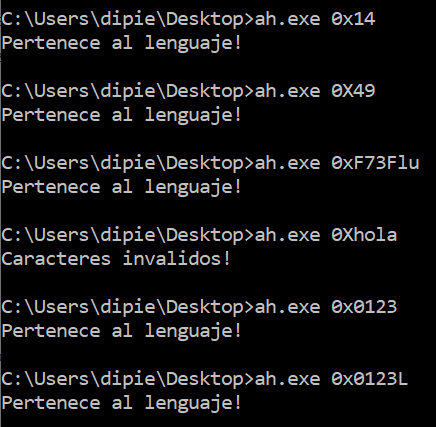
\includegraphics{images/automataHexa.PNG}
  \caption{Autómata reconocedor de constantes hexadecimales en consola}
  \label{fig:hexa-consola}
\end{figure}

\begin{figure}[b]
    \centering
    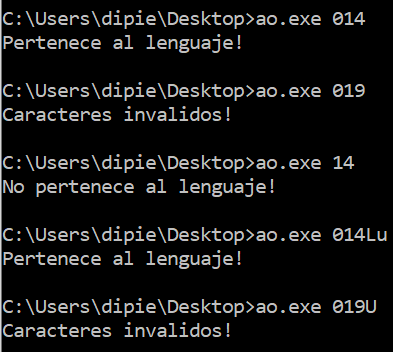
\includegraphics{automataOctal.PNG}
    \caption{Ejecución en consola de autómata octal}
    \label{fig:octal-consola}
\end{figure}

Se puede ver estos programas en funcionamiento en las imágenes \ref{fig:hexa-consola} y \ref{fig:octal-consola} en la página \pageref{fig:hexa-consola}, así como el programa que reconoce constantes decimales en la figura \ref{fig:decimal-consola} (página \pageref{fig:decimal-consola}).

Este último, como además retorna el valor numérico de la constante y esto corresponde a la resolución del problema desarrollado en la sección \ref{ej-valordecimal}, se explicará oportunamente allí.

\vspace{1cm}

\subsection{Programa que determina tipo de constante}
\label{ej-reconocedor}
\medbreak

Para realizar el programa que dada una constante reconoce de qué tipo es (si es válida), armamos una pequeña biblioteca con los autómatas del punto anterior. Veamos brevemente cómo luce el archivo \textit{header}:

\lstinputlisting[style=CStyle]{programas/constantes.h}

Lo lógico es intentar evaluar si la constante es octal, hexadecimal, o decimal utilizando las funciones \texttt{automataOctal(), automataHexa(), automataDecimal()}. \\
Como estos tres lenguajes tienen intersección vacía entre ellos (es decir, no hay ninguna constante que pertenezca a más de uno de estos lenguajes a la vez), esto se puede hacer sin problemas.\footnote{El ``0" debería reconocerse como constante octal de acuerdo a la gramática presentada, pero el valor de este número es en realidad el mismo en cualquier base. Además, no se tomó en cuenta este número para nuestra implementación de los autómatas, por lo que figuraría como ``constante inválida'' de ingresarse en este programa.}

La definición de las funciones en el archivo \texttt{constantes.c} que corresponde a este encabezado está \hyperref[constantesc]{incluida en el anexo}, página \pageref{anexo}.

El programa principal simplemente consta de una serie de bucles \texttt{if} que evalúan la pertenencia de la constante ingresada como argumento a los lenguajes que definimos.

\lstinputlisting[style=CStyle]{programas/reconocedorConstantes.c}

Entonces, al ingresar una constante, el programa mostrará en pantalla un mensaje indicando a qué tipo de constantes pertenece, o si no es válida en absoluto. \\
Este programa reconoce constantes hexadecimales, decimales y octales, en los tres casos soportando implementación signada y con sufijos. \\
Su funcionamiento en consola se puede ver en la imagen \ref{fig:reconocedor-constantes}, en la página \pageref{fig:reconocedor-constantes}.

\begin{figure}[b]
    \centering
    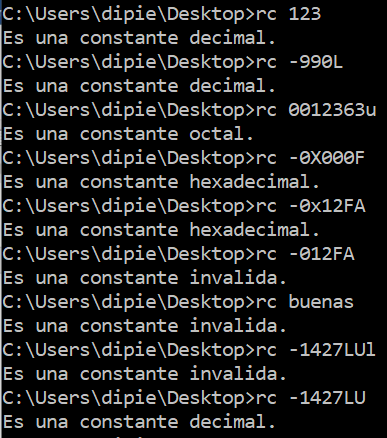
\includegraphics{images/reconocedorConstantes.PNG}
    \caption{Reconocedor de constantes, ejecución en consola}
    \label{fig:reconocedor-constantes}
\end{figure}

\bigskip

\subsection{Programa que retorna valor decimal de constante decimal}
\label{ej-valordecimal}
\medbreak

Este programa fue realizado originalmente para la resolución parcial del punto \ref{ej-constantes}, y fue posteriormente modificado para permitir el retorno del valor numérico de la constante ingresada como cadena de texto.

Si el programa lee un carácter, y el mismo es un dígito, entonces realiza la asignación

\begin{center}
    \texttt{num = num*10 + (carácter - '0');}
\end{center}

a una variable tipo entera \texttt{num} inicializada en 0.

Esto se vale de algunos "trucos":
\begin{itemize}
    \item Multiplicar un entero por su base y sumarle una cifra equivale a realizar una concatenación de un símbolo al final de una cadena de caracteres.
    \item El valor ASCII de las cifras numéricas es consecutivo, por lo que al restarle \texttt{'0'} obtenemos el desplazamiento desde el 0, es decir, por definición, su valor numérico.
\end{itemize}

Además, si el primer carácter leído es el símbolo \texttt{-}, una variable llamada ``signo" guarda el valor \texttt{-1}. Esa misma variable se inicializa en \texttt{1} para mantener el signo positivo en el caso de que la cadena represente un número positivo.

Posteriormente, al terminar la lectura de la cadena, se multiplica el valor almacenado en \texttt{num} por el valor almacenado en \texttt{signo} para conformar el valor final correcto.

Por lo tanto, el programa modificado para implementar el retorno del valor numérico de la constante luce como se muestra a continuación.

\newpage

\lstinputlisting[style=CStyle]{programas/decimal_limpiado.c}

En la línea 19 se realiza la actualización de \texttt{num} ante la presencia de un dígito, y en la 20 el análisis del signo. Finalmente, en la línea 23 se opera y se almacena el valor final signado.

Su funcionamiento se muestra en la imagen \ref{fig:decimal-consola}, página \pageref{fig:decimal-consola}.

\begin{figure}[b]
    \centering
    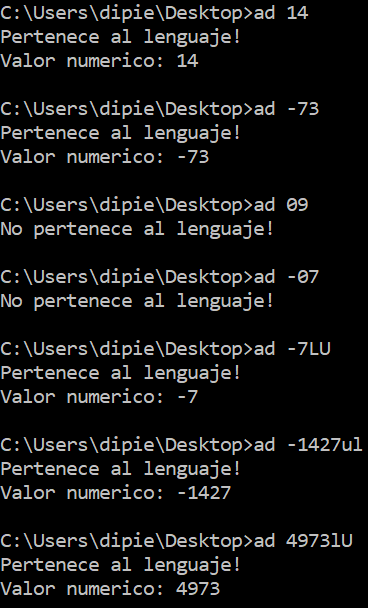
\includegraphics{images/automataDecimal2.PNG}
    \caption{Autómata decimal que además retorna valor numérico de las constantes, en consola}
    \label{fig:decimal-consola}
\end{figure}


\subsection{Programa que resuelve operación aritmética simple}
\label{ej-operacion}
\medbreak

Primero y principal, elaboramos la tabla de transiciones del lenguaje que describimos en la sección \ref{teoria}. El alfabeto son los dígitos del 0 al 9, y las 4 operaciones básicas: \texttt{+, -, *, /}.

También incluimos el dígrafo.

\begin{center}
    \begin{tabular}{||l c c c c c c||}
        \hline
        E & díg & + & - & * & / & 0\\
        \hline\hline
        q0- &1&5&5&5&5&1 \\ \hline
        q1  &1&2&2&2&3&1 \\ \hline
        q2  &4&5&5&5&5&4 \\ \hline
        q3  &4&5&5&5&5&5 \\ \hline
        q4+ &4&5&5&5&5&4 \\ \hline
        q5  &5&5&5&5&5&5 \\ \hline
    \end{tabular}
\end{center}
\medskip
\begin{center}
    \begin{tikzpicture}[scale=0.2]
        \tikzstyle{every node}+=[inner sep=0pt]
        \draw [black] (4.1,-27) circle (3);
        \draw (4.1,-27) node {$q0-$};
        \draw [black] (16.2,-27) circle (3);
        \draw (16.2,-27) node {$q1$};
        \draw [black] (28.6,-27) circle (3);
        \draw (28.6,-27) node {$q2$};
        \draw [black] (28.6,-37.3) circle (3);
        \draw (28.6,-37.3) node {$q3$};
        \draw [black] (41.6,-27) circle (3);
        \draw (41.6,-27) node {$q4$};
        \draw [black] (41.6,-27) circle (2.4);
        \draw [black] (58.6,-27) circle (3);
        \draw (58.6,-27) node {$q5$};
        \draw [black] (-0.1,-27) -- (1.1,-27);
        \fill [black] (1.1,-27) -- (0.3,-26.5) -- (0.3,-27.5);
        \draw [black] (7.1,-27) -- (13.2,-27);
        \fill [black] (13.2,-27) -- (12.4,-26.5) -- (12.4,-27.5);
        \draw (10.15,-26.5) node [above] {$0|dig$};
        \draw [black] (14.877,-24.32) arc (234:-54:2.25);
        \draw (16.2,-19.75) node [above] {$0|dig$};
        \fill [black] (17.52,-24.32) -- (18.4,-23.97) -- (17.59,-23.38);
        \draw [black] (19.2,-27) -- (25.6,-27);
        \fill [black] (25.6,-27) -- (24.8,-26.5) -- (24.8,-27.5);
        \draw (22.4,-26.5) node [above] {\footnotesize $+|-|*$};
        \draw [black] (18.51,-28.92) -- (26.29,-35.38);
        \fill [black] (26.29,-35.38) -- (26,-34.49) -- (25.36,-35.26);
        \draw (21.61,-32.64) node [below] {$/$};
        \draw [black] (31.6,-27) -- (38.6,-27);
        \fill [black] (38.6,-27) -- (37.8,-26.5) -- (37.8,-27.5);
        \draw (35.1,-26.5) node [above] {$0|dig$};
        \draw [black] (30.95,-35.44) -- (39.25,-28.86);
        \fill [black] (39.25,-28.86) -- (38.31,-28.97) -- (38.93,-29.75);
        \draw (33.32,-33.65) node [above] {\rotatebox{42}{{$dig$}}};
        \draw [black] (40.277,-24.32) arc (234:-54:2.25);
        \draw (41.6,-19.75) node [above] {$0|dig$};
        \fill [black] (42.92,-24.32) -- (43.8,-23.97) -- (42.99,-23.38);
        \draw [black] (44.6,-27) -- (55.6,-27);
        \fill [black] (55.6,-27) -- (54.8,-26.5) -- (54.8,-27.5);
        \draw (50.1,-26.5) node [above] {$+|-|*|/$};
        \draw [black] (31.44,-36.33) -- (55.76,-27.97);
        \fill [black] (55.76,-27.97) -- (54.84,-27.76) -- (55.17,-28.71);
        \draw (44,-31) node [below] {\rotatebox{18}{{$+|-|*|/|0$}}};
        \draw [black] (29.67,-24.202) arc (153.54464:26.45536:15.559);
        \fill [black] (57.53,-24.2) -- (57.62,-23.26) -- (56.73,-23.71);
        \draw (43.6,-15.07) node [above] {$+|-|*|/$};
        \draw [black] (4.853,-24.097) arc (162.37447:17.62553:27.803);
        \fill [black] (57.85,-24.1) -- (58.08,-23.18) -- (57.13,-23.49);
        \draw (31.35,-4.21) node [above] {$+|-|*|/$};
        \draw [black] (58.552,-24.012) arc (208.65382:-79.34618:2.25);
        \draw (61.37,-20.37) node [above] {$(!)$}; %0|dig|+|-|*|/
        \fill [black] (60.94,-25.14) -- (61.88,-25.2) -- (61.4,-24.32);
    \end{tikzpicture}
\end{center}

Utilizando una lógica similar a la del programa en la consigna ``\nameref{ej-valordecimal}", pero ahora utilizando la información brindada por la variable \texttt{estado}, almacenamos los valores de ambos operandos.

Comenzamos con la definición de la función \texttt{opercionAritmetica()} que dada una cadena retorna el valor de evaluarla, si es una operación válida de la forma \texttt{[num][operando][num]}. \\
Se estructura prácticamente de la misma forma que las funciones \texttt{automataX()} de los reconocedores de octal, hexadecimal, y decimal.

La diferencia en este programa es que mientras el estado sea igual a 1, se almacenará el valor numérico en la variable \texttt{num1}, pero si el valor es en cambio 4, se almacenará en \texttt{num2} (ver líneas 24 y 26).

Asimismo, si el estado es el 2 o el 3, significa que se ingresó un operando, y este se almacenará en la variable \texttt{operador} (línea 25).

El autómata fue diseñado para que rechace todas las palabras que incluyan la secuencia \verb|"/0"|, así que no es necesario incluir un bucle \texttt{if} que se fije en eso (línea 35).

Veamos el programa a continuación.

\lstinputlisting[style=CStyle]{programas/aritmetica.c}

El resultado de la operación evaluada según el operador almacenado (líneas 32 a 35) se almacena en la dirección apuntada por el puntero pasado como argumento (línea 39). \footnote{No era necesario usar la variable \texttt{num3} pero lo hicimos igualmente por cuestiones de organización personal.}

Finalmente, el \texttt{main()} es muy sencillo y luce así:

\lstinputlisting[style=CStyle]{programas/aritmetica_main.c}

El programa se muestra funcionando correctamente en la figura \ref{fig:aritmetica-consola}, página \pageref{fig:aritmetica-consola}.

\begin{figure}[b]
    \centering
    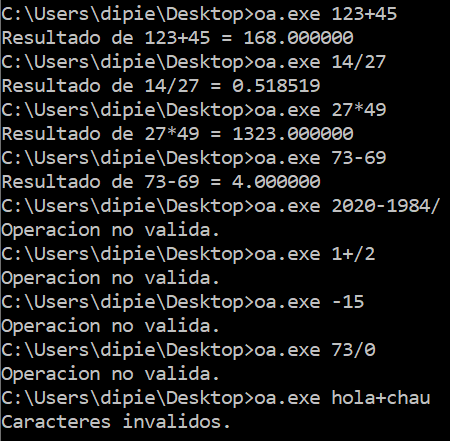
\includegraphics{images/operacionesAritmeticas.PNG}
    \caption{Autómata que reconoce y evalúa una operación aritmética simple}
    \label{fig:aritmetica-consola}
\end{figure}

\section{Conclusiones}
\label{conclusiones}

Hemos confeccionado nuestra propia versión de algunos de los lenguajes regulares que componen la totalidad del lenguaje ANSI C, así como realizado programas a modo de ejemplo para probar su correcto funcionamiento.

Además, vimos que las expresiones aritméticas más simples (constando únicamente de dos enteros y un operando en notación infija) también se pueden representar como un lenguaje regular.

Pudimos practicar el diseño de autómatas finitos, y el manejo del lenguaje C.

%%% Anexo %%%
\newpage
\section{Anexo} \label{anexo}
\bigbreak
\subsection{Definición de funciones del archivo de cabecera \texttt{constantes.h}} \label{constantesc}
\lstinputlisting[style=CStyle]{programas/constantes.c}

\subsection{Repositorio en GitHub}
\label{repo}

Utilizamos esta herramienta para llevar cuenta de los cambios realizados en cada uno de los programas.

\begin{center}
\url{https://github.com/GuidoDipietro/tpAutomatas}
\end{center}

\end{document}